\section{Introduction}
\label{sec:introduction}
%\note{The importance of gas sensors is made clear. I.e. the need for them in the civil, industrial, medical and military sector. An overview of conventional gas sensors is given. I.e. Bulk-MOX, NDIR, catalytic bead sensor. Novel gas sensors based on 2D structures are presented. Their advantages (small size, flexibility, CMOS-compatibility, sensitivity, specificity) is discussed. Multiple 2D gas sensors are shortly presented. Eventually gas sensors based on 2D TMD heterojunctions are motivated.}

Gas sensing has been used by humans even before the advent of electronic engineering. A prominent example are birds, which accompanied miners in the shafts. If the birds stopped chirping, it was the signal that the oxygen in the air has been replaced by other gases and that the cave should be evacuated as soon as possible \cite{nrc1991}. Since then, gas sensors have evolved drastically, and are now mostly free of any animal cruelty. Today gas sensors are not only used for sensing air quality in underground caves, but are also applied in industrial processes \cite{Johny2016, Wang2017}, in medical fields \cite{Eamsaard2016, Wilson2018}, on military battlefields \cite{Kumar2020a} or are used to sense the gas composition of the environment \cite{Harrou2018}. In the sense of ubiquitous sensing, there is the demand that these sensor become smaller, faster and more power efficient. Trends in that direction allow the development of more efficient industrial processes, increase the efficiency of the medical care or allow precise warnings on the battle field \cite{Wang2022, Kumar2020, Mathew2021}. Market predictions, like the one presented in \cref{fig:gas_sensor_market} confirm this development. \\
\begin{figure}
\centering
    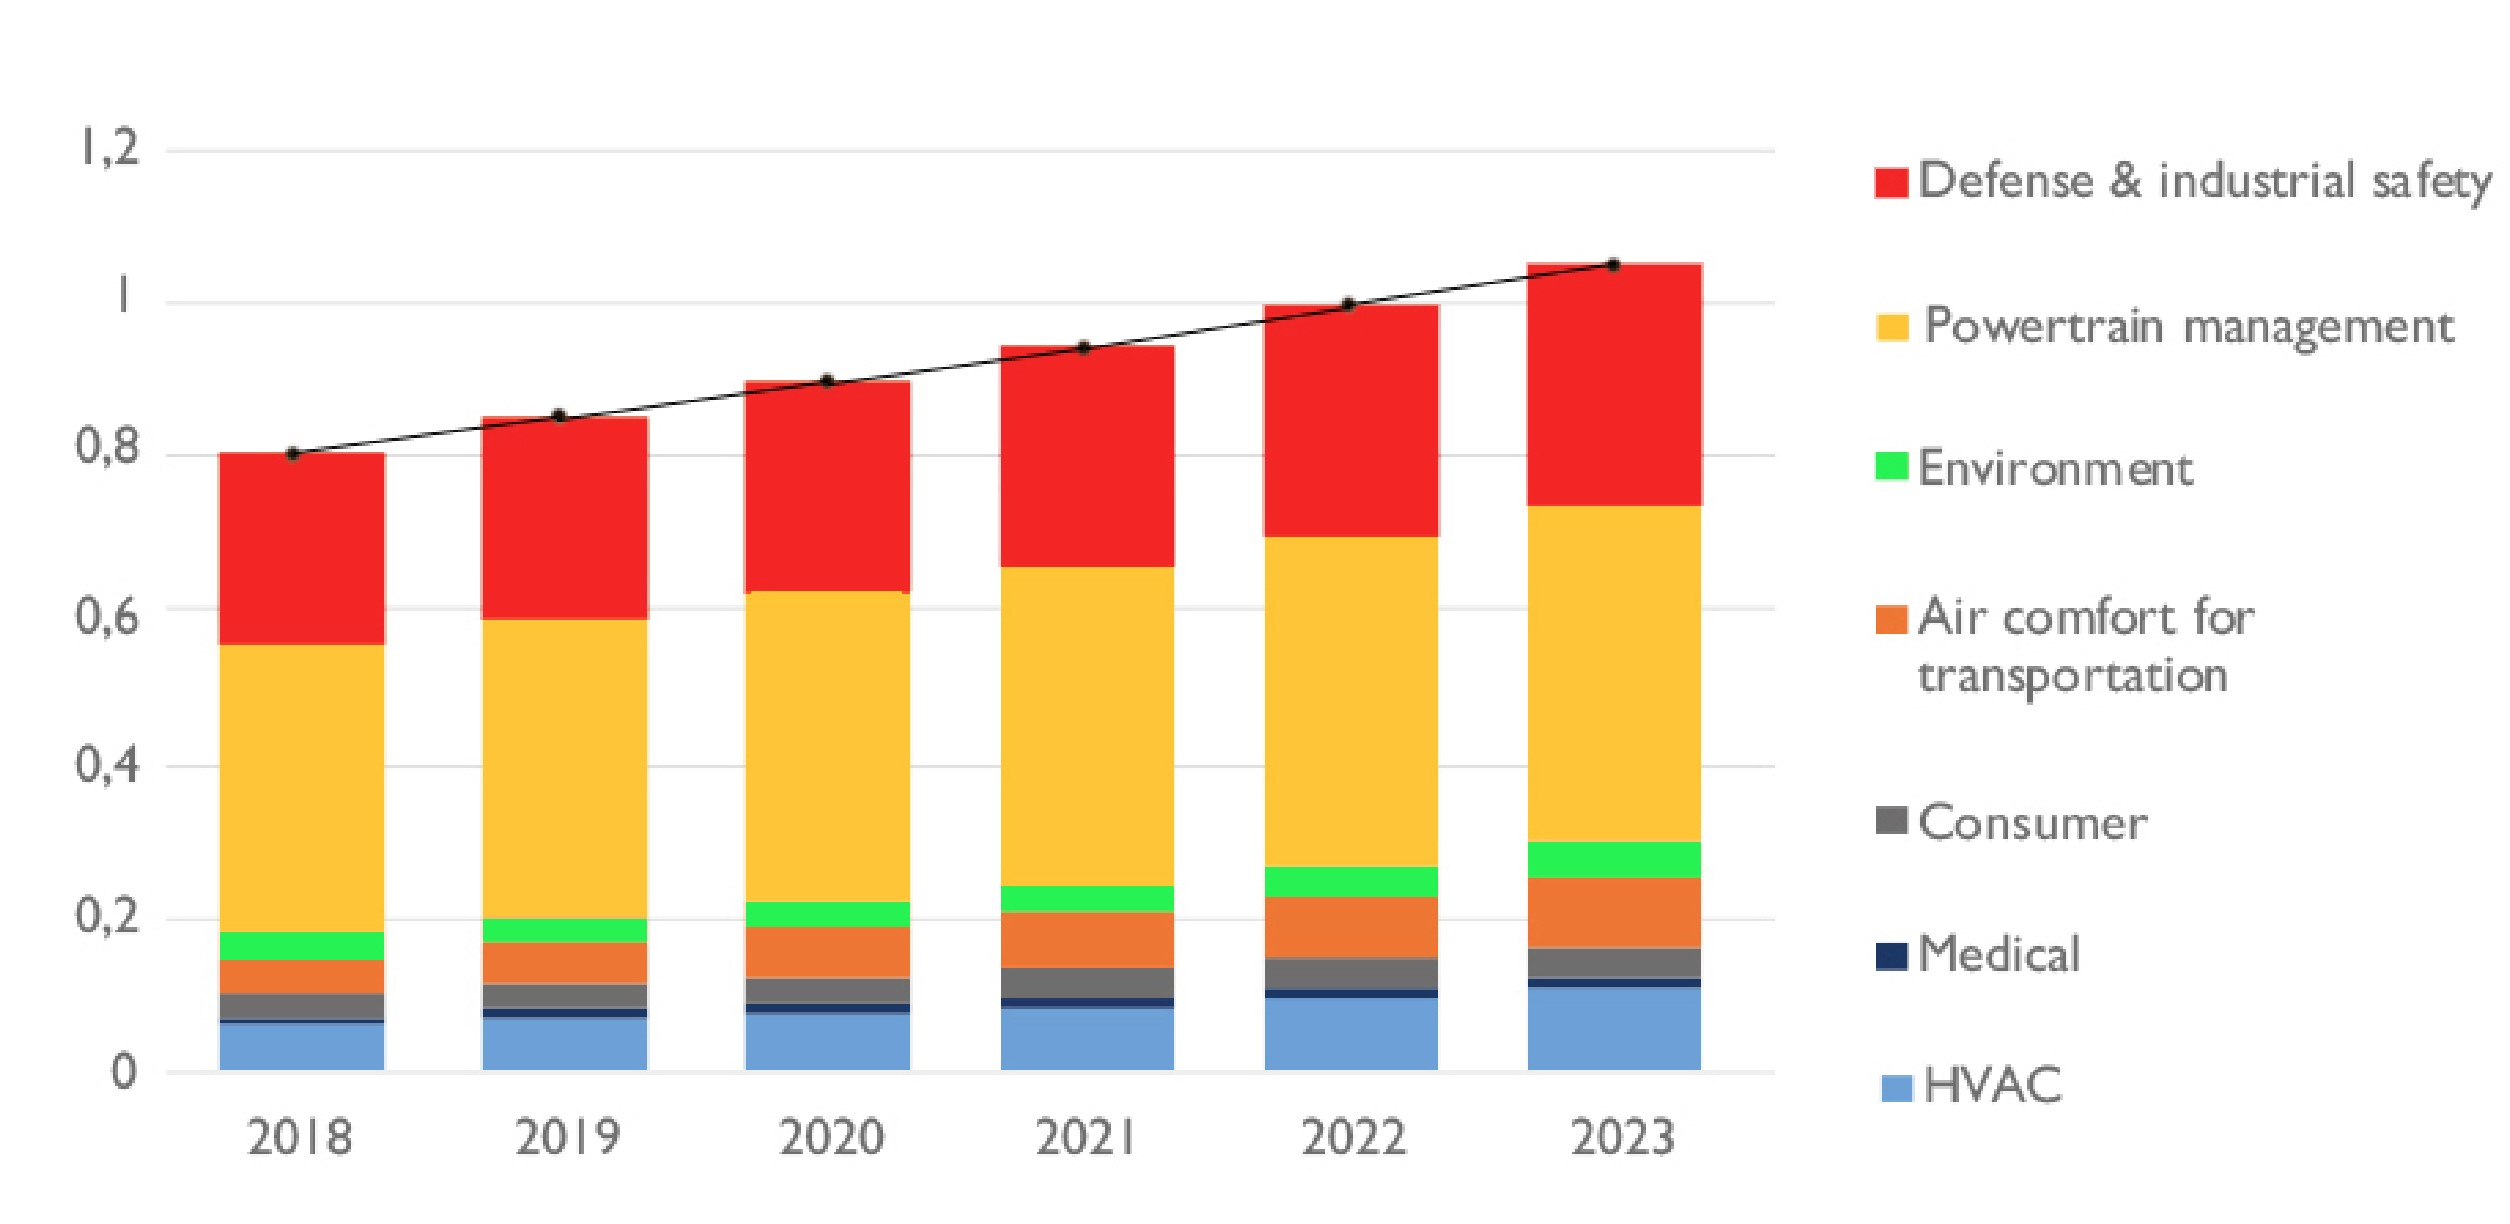
\includegraphics[width=\textwidth]{01_introduction/fig/gas_sensor_market.jpg}
    \caption{The expected market development, as predicted by \cite{yole2021}. Vertical axis is in billion dollars.}
    \label{fig:gas_sensor_market}
\end{figure}
There are a variety of types of gas sensors, whose measurement principles range from optical sensing to chemical effects. One of the most popular gas sensor is the carbon monoxide (CO) sensor, which in many countries is nowadays mandatory to be installed in households \cite{ncsl2018}. The most common version of this sensor is based on a fuel cell like reaction, which generates an electrical current. This current is highly proportional to the CO concentration in the air. This sensor allows detection of concentrations as low as tenths of ppb. First symptoms of carbon monoxide poisoning start at 35 ppm \cite{Goldstein2008}. \\
Another sensor principle relies on the adsorption of the analyte on the surface of a metal oxide bulk structure. The analyte then exchanges electrons with the bulk and modulates its conductivity. This effect serves as metric for the concentration of the analyte in the vicinity of the sensor. The sensor can be made quite small, however it has to heated up to around \SI{400}{\celsius}, so that the adsorption effect takes place. The Taguchi sensor (type TGS 813) \cite{Yamauchi2012, Hartman2021}  is quite popular and its use is very widespread. The Taguchi sensor is sensitive to combustible gases (propan, butan, methan) and can sense concentrations as low as 500 ppm. \\
Another sensor principle is \gls{ndir}. The sensor analyzes the spectrum of light, that is transmitted through the analyte. As most gases have a very specific transmittivity spectrum, and the light spectrum of the source is known, the type and concentration of the analyte gas can be determined. This sensor has the major advantage, that it is able to detect various different gases, where as other sensors are only sensitive to single types of gases. However, the sensor requires long interferometer lengths, and is therefore quite bulky. Such sensor come with a an accuracy of 50 ppm \cite{lp8} (for instance for the gas carbon dioxide). \\
Recent market studies\cite{yole2021, Buckley2020} suggest, that by far the most abundant gas sensor type is the electrochemical one, followed by \gls{ndir} types. The large market shares of these two types can be explained through their good selectivity and relatively low cost. \Cref{fig:gas_sensor_distribution} depicts the relative market revenues, split according to gas sensor type. It can be seen, that 2D materials do not appear in this statistic, which implies that they are not yet feasible for mass market. This paper tries to identify the reasons for that circumstance. \\
\begin{figure}
\centering
    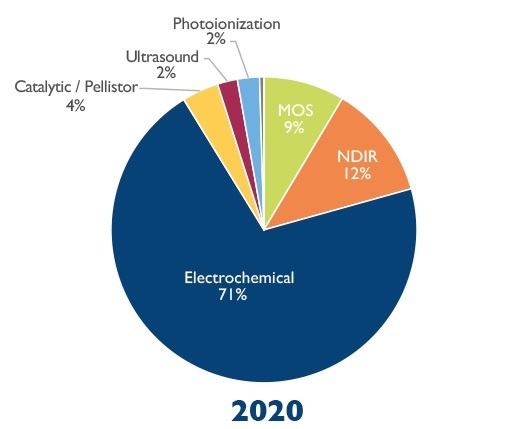
\includegraphics[width=.5\textwidth]{01_introduction/fig/gas_sensor_distribution.jpg}
    \caption{The distribution of gas sensor operating principles \cite{yole2021}.}
    \label{fig:gas_sensor_distribution}
\end{figure}
Great scientific efforts have been undertaken to find new sensing principles that allow further miniaturization and lowering of the power consumption of the sensors. In the last two decades, ample expectations have been made with regards to graphene-based sensors. Scientists believed, that the extreme surface to volume ratio favors a higher sensitivity to gases. Ultimately this assumption could not be satisfied \cite{Geim2013}. One of the major reasons was the lacking band gap of the material. However, progresses in fabrication methods allowed the efficient production of other 2D structures, which exposed the properties, that have been desired from graphene. In \cite{He2012}, one of the first two-dimensional, MoS2 based sensors have been proposed. The device provided a sensitivity of \SI{18}{\percent} at 5 ppm NO2 and a relaxation time of \SI{30}{\minute}. As it was fabricated as a \gls{tft} device on a flexible substrate, it could be bent, without being destroyed. This property enables the integration of the sensor into wearable devices. In \cite{Long2016} a different approach has been followed. A few-layered MoS2 film has been deposited onto a graphene hybrid aerogel scaffold. This device provides a lower detection limit of 50 ppb and a relaxation time of \SI{1}{\minute} (when heated to \SI{200}{\celsius}). \\
These two examples shall testify, that remarkable effects can be shown with 2D structures. One of the most promising material systems is the familiy of \glspl{tmd}. They show strong sensitivity to gas exposure and have an acceptable recovery time. However, one of its most intriguing properties is the potential compatibility to \gls{cmos} fabrication processes. This feature enables the integration of the sensor onto the same silicon wafer as \gls{cmos} transistors. In extension, this implies that the sensor can be integrated onto the same die as its signal conditioning circuits and the digital processing. Effectively, this would cut down on fabrication costs and enable highly integrated gas sensing solutions. Due to these fascinating promises, this publication shall shine a light on gas sensor based on 2D \gls{tmd} structures. \Cref{sec:functionality} explains the workings of 2D \glspl{tmd}. After that, the current fabrication methods are layed out in \cref{sec:fabrication}. In order to give an overview above the tunable parameters of 2D \glspl{tmd}, in \cref{sec:2d_tmd_heterojunction_gas_sensors} two different sensor implementations are compared and discussed. Eventually, a summary and outlook is given in \cref{sec:conclusion}.